\begin{figure}[htbp]
\centering
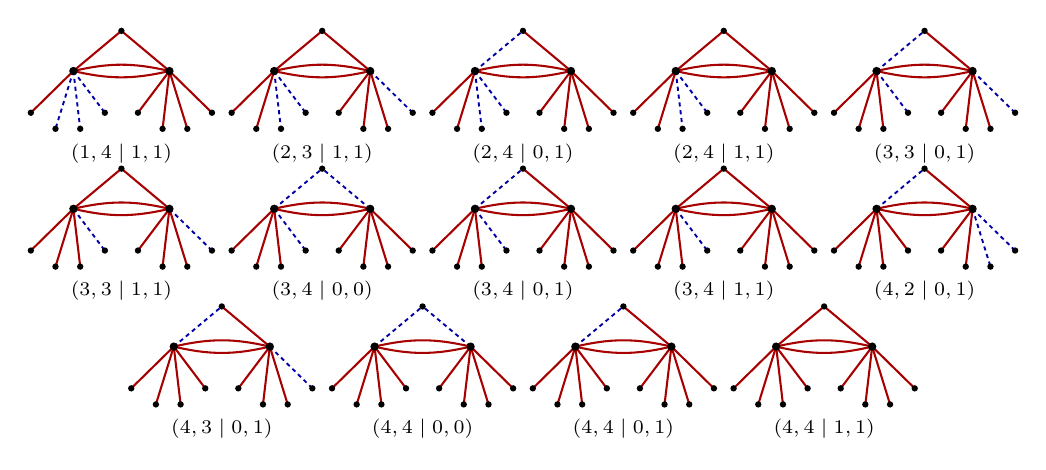
\begin{tikzpicture}[font=\scriptsize,
sc marked/.style={draw=red!65!black,line width=.75pt},
sc unmarked/.style={draw=blue!65!black,line width=.68pt,dash pattern=on 1.5pt off 1.35pt}]
\begin{scope}[shift={(-5.1,0)}]
\coordinate (u) at (-0.61,0.03);
\coordinate (v) at (0.61,0.03);
\coordinate (u0) at (-1.15,-0.5);
\coordinate (u1) at (-0.837,-0.704);
\coordinate (u2) at (-0.523,-0.704);
\coordinate (u3) at (-0.21,-0.5);
\coordinate (v0) at (0.21,-0.5);
\coordinate (v1) at (0.523,-0.704);
\coordinate (v2) at (0.837,-0.704);
\coordinate (v3) at (1.15,-0.5);
\coordinate (w) at (0,0.54);
\draw[sc marked] (u) to[bend left=13] (v);
\draw[sc marked] (u) to[bend right=13] (v);
\draw[sc marked] (u) -- (u0);
\draw[sc unmarked] (u) -- (u1);
\draw[sc unmarked] (u) -- (u2);
\draw[sc unmarked] (u) -- (u3);
\draw[sc marked] (v) -- (v0);
\draw[sc marked] (v) -- (v1);
\draw[sc marked] (v) -- (v2);
\draw[sc marked] (v) -- (v3);
\draw[sc marked] (u) -- (w);
\draw[sc marked] (v) -- (w);
\fill (u) circle[radius=1.5pt];
\fill (v) circle[radius=1.5pt];
\fill (u0) circle[radius=1.15pt];
\fill (u1) circle[radius=1.15pt];
\fill (u2) circle[radius=1.15pt];
\fill (u3) circle[radius=1.15pt];
\fill (v0) circle[radius=1.15pt];
\fill (v1) circle[radius=1.15pt];
\fill (v2) circle[radius=1.15pt];
\fill (v3) circle[radius=1.15pt];
\fill (w) circle[radius=1.15pt];
\node[anchor=north,inner sep=1pt] at (0,-.85) {\((1,4\mid 1,1)\)};
\end{scope}
\begin{scope}[shift={(-2.55,0)}]
\coordinate (u) at (-0.61,0.03);
\coordinate (v) at (0.61,0.03);
\coordinate (u0) at (-1.15,-0.5);
\coordinate (u1) at (-0.837,-0.704);
\coordinate (u2) at (-0.523,-0.704);
\coordinate (u3) at (-0.21,-0.5);
\coordinate (v0) at (0.21,-0.5);
\coordinate (v1) at (0.523,-0.704);
\coordinate (v2) at (0.837,-0.704);
\coordinate (v3) at (1.15,-0.5);
\coordinate (w) at (0,0.54);
\draw[sc marked] (u) to[bend left=13] (v);
\draw[sc marked] (u) to[bend right=13] (v);
\draw[sc marked] (u) -- (u0);
\draw[sc marked] (u) -- (u1);
\draw[sc unmarked] (u) -- (u2);
\draw[sc unmarked] (u) -- (u3);
\draw[sc marked] (v) -- (v0);
\draw[sc marked] (v) -- (v1);
\draw[sc marked] (v) -- (v2);
\draw[sc unmarked] (v) -- (v3);
\draw[sc marked] (u) -- (w);
\draw[sc marked] (v) -- (w);
\fill (u) circle[radius=1.5pt];
\fill (v) circle[radius=1.5pt];
\fill (u0) circle[radius=1.15pt];
\fill (u1) circle[radius=1.15pt];
\fill (u2) circle[radius=1.15pt];
\fill (u3) circle[radius=1.15pt];
\fill (v0) circle[radius=1.15pt];
\fill (v1) circle[radius=1.15pt];
\fill (v2) circle[radius=1.15pt];
\fill (v3) circle[radius=1.15pt];
\fill (w) circle[radius=1.15pt];
\node[anchor=north,inner sep=1pt] at (0,-.85) {\((2,3\mid 1,1)\)};
\end{scope}
\begin{scope}[shift={(0,0)}]
\coordinate (u) at (-0.61,0.03);
\coordinate (v) at (0.61,0.03);
\coordinate (u0) at (-1.15,-0.5);
\coordinate (u1) at (-0.837,-0.704);
\coordinate (u2) at (-0.523,-0.704);
\coordinate (u3) at (-0.21,-0.5);
\coordinate (v0) at (0.21,-0.5);
\coordinate (v1) at (0.523,-0.704);
\coordinate (v2) at (0.837,-0.704);
\coordinate (v3) at (1.15,-0.5);
\coordinate (w) at (0,0.54);
\draw[sc marked] (u) to[bend left=13] (v);
\draw[sc marked] (u) to[bend right=13] (v);
\draw[sc marked] (u) -- (u0);
\draw[sc marked] (u) -- (u1);
\draw[sc unmarked] (u) -- (u2);
\draw[sc unmarked] (u) -- (u3);
\draw[sc marked] (v) -- (v0);
\draw[sc marked] (v) -- (v1);
\draw[sc marked] (v) -- (v2);
\draw[sc marked] (v) -- (v3);
\draw[sc unmarked] (u) -- (w);
\draw[sc marked] (v) -- (w);
\fill (u) circle[radius=1.5pt];
\fill (v) circle[radius=1.5pt];
\fill (u0) circle[radius=1.15pt];
\fill (u1) circle[radius=1.15pt];
\fill (u2) circle[radius=1.15pt];
\fill (u3) circle[radius=1.15pt];
\fill (v0) circle[radius=1.15pt];
\fill (v1) circle[radius=1.15pt];
\fill (v2) circle[radius=1.15pt];
\fill (v3) circle[radius=1.15pt];
\fill (w) circle[radius=1.15pt];
\node[anchor=north,inner sep=1pt] at (0,-.85) {\((2,4\mid 0,1)\)};
\end{scope}
\begin{scope}[shift={(2.55,0)}]
\coordinate (u) at (-0.61,0.03);
\coordinate (v) at (0.61,0.03);
\coordinate (u0) at (-1.15,-0.5);
\coordinate (u1) at (-0.837,-0.704);
\coordinate (u2) at (-0.523,-0.704);
\coordinate (u3) at (-0.21,-0.5);
\coordinate (v0) at (0.21,-0.5);
\coordinate (v1) at (0.523,-0.704);
\coordinate (v2) at (0.837,-0.704);
\coordinate (v3) at (1.15,-0.5);
\coordinate (w) at (0,0.54);
\draw[sc marked] (u) to[bend left=13] (v);
\draw[sc marked] (u) to[bend right=13] (v);
\draw[sc marked] (u) -- (u0);
\draw[sc marked] (u) -- (u1);
\draw[sc unmarked] (u) -- (u2);
\draw[sc unmarked] (u) -- (u3);
\draw[sc marked] (v) -- (v0);
\draw[sc marked] (v) -- (v1);
\draw[sc marked] (v) -- (v2);
\draw[sc marked] (v) -- (v3);
\draw[sc marked] (u) -- (w);
\draw[sc marked] (v) -- (w);
\fill (u) circle[radius=1.5pt];
\fill (v) circle[radius=1.5pt];
\fill (u0) circle[radius=1.15pt];
\fill (u1) circle[radius=1.15pt];
\fill (u2) circle[radius=1.15pt];
\fill (u3) circle[radius=1.15pt];
\fill (v0) circle[radius=1.15pt];
\fill (v1) circle[radius=1.15pt];
\fill (v2) circle[radius=1.15pt];
\fill (v3) circle[radius=1.15pt];
\fill (w) circle[radius=1.15pt];
\node[anchor=north,inner sep=1pt] at (0,-.85) {\((2,4\mid 1,1)\)};
\end{scope}
\begin{scope}[shift={(5.1,0)}]
\coordinate (u) at (-0.61,0.03);
\coordinate (v) at (0.61,0.03);
\coordinate (u0) at (-1.15,-0.5);
\coordinate (u1) at (-0.837,-0.704);
\coordinate (u2) at (-0.523,-0.704);
\coordinate (u3) at (-0.21,-0.5);
\coordinate (v0) at (0.21,-0.5);
\coordinate (v1) at (0.523,-0.704);
\coordinate (v2) at (0.837,-0.704);
\coordinate (v3) at (1.15,-0.5);
\coordinate (w) at (0,0.54);
\draw[sc marked] (u) to[bend left=13] (v);
\draw[sc marked] (u) to[bend right=13] (v);
\draw[sc marked] (u) -- (u0);
\draw[sc marked] (u) -- (u1);
\draw[sc marked] (u) -- (u2);
\draw[sc unmarked] (u) -- (u3);
\draw[sc marked] (v) -- (v0);
\draw[sc marked] (v) -- (v1);
\draw[sc marked] (v) -- (v2);
\draw[sc unmarked] (v) -- (v3);
\draw[sc unmarked] (u) -- (w);
\draw[sc marked] (v) -- (w);
\fill (u) circle[radius=1.5pt];
\fill (v) circle[radius=1.5pt];
\fill (u0) circle[radius=1.15pt];
\fill (u1) circle[radius=1.15pt];
\fill (u2) circle[radius=1.15pt];
\fill (u3) circle[radius=1.15pt];
\fill (v0) circle[radius=1.15pt];
\fill (v1) circle[radius=1.15pt];
\fill (v2) circle[radius=1.15pt];
\fill (v3) circle[radius=1.15pt];
\fill (w) circle[radius=1.15pt];
\node[anchor=north,inner sep=1pt] at (0,-.85) {\((3,3\mid 0,1)\)};
\end{scope}
\begin{scope}[shift={(-5.1,-1.75)}]
\coordinate (u) at (-0.61,0.03);
\coordinate (v) at (0.61,0.03);
\coordinate (u0) at (-1.15,-0.5);
\coordinate (u1) at (-0.837,-0.704);
\coordinate (u2) at (-0.523,-0.704);
\coordinate (u3) at (-0.21,-0.5);
\coordinate (v0) at (0.21,-0.5);
\coordinate (v1) at (0.523,-0.704);
\coordinate (v2) at (0.837,-0.704);
\coordinate (v3) at (1.15,-0.5);
\coordinate (w) at (0,0.54);
\draw[sc marked] (u) to[bend left=13] (v);
\draw[sc marked] (u) to[bend right=13] (v);
\draw[sc marked] (u) -- (u0);
\draw[sc marked] (u) -- (u1);
\draw[sc marked] (u) -- (u2);
\draw[sc unmarked] (u) -- (u3);
\draw[sc marked] (v) -- (v0);
\draw[sc marked] (v) -- (v1);
\draw[sc marked] (v) -- (v2);
\draw[sc unmarked] (v) -- (v3);
\draw[sc marked] (u) -- (w);
\draw[sc marked] (v) -- (w);
\fill (u) circle[radius=1.5pt];
\fill (v) circle[radius=1.5pt];
\fill (u0) circle[radius=1.15pt];
\fill (u1) circle[radius=1.15pt];
\fill (u2) circle[radius=1.15pt];
\fill (u3) circle[radius=1.15pt];
\fill (v0) circle[radius=1.15pt];
\fill (v1) circle[radius=1.15pt];
\fill (v2) circle[radius=1.15pt];
\fill (v3) circle[radius=1.15pt];
\fill (w) circle[radius=1.15pt];
\node[anchor=north,inner sep=1pt] at (0,-.85) {\((3,3\mid 1,1)\)};
\end{scope}
\begin{scope}[shift={(-2.55,-1.75)}]
\coordinate (u) at (-0.61,0.03);
\coordinate (v) at (0.61,0.03);
\coordinate (u0) at (-1.15,-0.5);
\coordinate (u1) at (-0.837,-0.704);
\coordinate (u2) at (-0.523,-0.704);
\coordinate (u3) at (-0.21,-0.5);
\coordinate (v0) at (0.21,-0.5);
\coordinate (v1) at (0.523,-0.704);
\coordinate (v2) at (0.837,-0.704);
\coordinate (v3) at (1.15,-0.5);
\coordinate (w) at (0,0.54);
\draw[sc marked] (u) to[bend left=13] (v);
\draw[sc marked] (u) to[bend right=13] (v);
\draw[sc marked] (u) -- (u0);
\draw[sc marked] (u) -- (u1);
\draw[sc marked] (u) -- (u2);
\draw[sc unmarked] (u) -- (u3);
\draw[sc marked] (v) -- (v0);
\draw[sc marked] (v) -- (v1);
\draw[sc marked] (v) -- (v2);
\draw[sc marked] (v) -- (v3);
\draw[sc unmarked] (u) -- (w);
\draw[sc unmarked] (v) -- (w);
\fill (u) circle[radius=1.5pt];
\fill (v) circle[radius=1.5pt];
\fill (u0) circle[radius=1.15pt];
\fill (u1) circle[radius=1.15pt];
\fill (u2) circle[radius=1.15pt];
\fill (u3) circle[radius=1.15pt];
\fill (v0) circle[radius=1.15pt];
\fill (v1) circle[radius=1.15pt];
\fill (v2) circle[radius=1.15pt];
\fill (v3) circle[radius=1.15pt];
\fill (w) circle[radius=1.15pt];
\node[anchor=north,inner sep=1pt] at (0,-.85) {\((3,4\mid 0,0)\)};
\end{scope}
\begin{scope}[shift={(0,-1.75)}]
\coordinate (u) at (-0.61,0.03);
\coordinate (v) at (0.61,0.03);
\coordinate (u0) at (-1.15,-0.5);
\coordinate (u1) at (-0.837,-0.704);
\coordinate (u2) at (-0.523,-0.704);
\coordinate (u3) at (-0.21,-0.5);
\coordinate (v0) at (0.21,-0.5);
\coordinate (v1) at (0.523,-0.704);
\coordinate (v2) at (0.837,-0.704);
\coordinate (v3) at (1.15,-0.5);
\coordinate (w) at (0,0.54);
\draw[sc marked] (u) to[bend left=13] (v);
\draw[sc marked] (u) to[bend right=13] (v);
\draw[sc marked] (u) -- (u0);
\draw[sc marked] (u) -- (u1);
\draw[sc marked] (u) -- (u2);
\draw[sc unmarked] (u) -- (u3);
\draw[sc marked] (v) -- (v0);
\draw[sc marked] (v) -- (v1);
\draw[sc marked] (v) -- (v2);
\draw[sc marked] (v) -- (v3);
\draw[sc unmarked] (u) -- (w);
\draw[sc marked] (v) -- (w);
\fill (u) circle[radius=1.5pt];
\fill (v) circle[radius=1.5pt];
\fill (u0) circle[radius=1.15pt];
\fill (u1) circle[radius=1.15pt];
\fill (u2) circle[radius=1.15pt];
\fill (u3) circle[radius=1.15pt];
\fill (v0) circle[radius=1.15pt];
\fill (v1) circle[radius=1.15pt];
\fill (v2) circle[radius=1.15pt];
\fill (v3) circle[radius=1.15pt];
\fill (w) circle[radius=1.15pt];
\node[anchor=north,inner sep=1pt] at (0,-.85) {\((3,4\mid 0,1)\)};
\end{scope}
\begin{scope}[shift={(2.55,-1.75)}]
\coordinate (u) at (-0.61,0.03);
\coordinate (v) at (0.61,0.03);
\coordinate (u0) at (-1.15,-0.5);
\coordinate (u1) at (-0.837,-0.704);
\coordinate (u2) at (-0.523,-0.704);
\coordinate (u3) at (-0.21,-0.5);
\coordinate (v0) at (0.21,-0.5);
\coordinate (v1) at (0.523,-0.704);
\coordinate (v2) at (0.837,-0.704);
\coordinate (v3) at (1.15,-0.5);
\coordinate (w) at (0,0.54);
\draw[sc marked] (u) to[bend left=13] (v);
\draw[sc marked] (u) to[bend right=13] (v);
\draw[sc marked] (u) -- (u0);
\draw[sc marked] (u) -- (u1);
\draw[sc marked] (u) -- (u2);
\draw[sc unmarked] (u) -- (u3);
\draw[sc marked] (v) -- (v0);
\draw[sc marked] (v) -- (v1);
\draw[sc marked] (v) -- (v2);
\draw[sc marked] (v) -- (v3);
\draw[sc marked] (u) -- (w);
\draw[sc marked] (v) -- (w);
\fill (u) circle[radius=1.5pt];
\fill (v) circle[radius=1.5pt];
\fill (u0) circle[radius=1.15pt];
\fill (u1) circle[radius=1.15pt];
\fill (u2) circle[radius=1.15pt];
\fill (u3) circle[radius=1.15pt];
\fill (v0) circle[radius=1.15pt];
\fill (v1) circle[radius=1.15pt];
\fill (v2) circle[radius=1.15pt];
\fill (v3) circle[radius=1.15pt];
\fill (w) circle[radius=1.15pt];
\node[anchor=north,inner sep=1pt] at (0,-.85) {\((3,4\mid 1,1)\)};
\end{scope}
\begin{scope}[shift={(5.1,-1.75)}]
\coordinate (u) at (-0.61,0.03);
\coordinate (v) at (0.61,0.03);
\coordinate (u0) at (-1.15,-0.5);
\coordinate (u1) at (-0.837,-0.704);
\coordinate (u2) at (-0.523,-0.704);
\coordinate (u3) at (-0.21,-0.5);
\coordinate (v0) at (0.21,-0.5);
\coordinate (v1) at (0.523,-0.704);
\coordinate (v2) at (0.837,-0.704);
\coordinate (v3) at (1.15,-0.5);
\coordinate (w) at (0,0.54);
\draw[sc marked] (u) to[bend left=13] (v);
\draw[sc marked] (u) to[bend right=13] (v);
\draw[sc marked] (u) -- (u0);
\draw[sc marked] (u) -- (u1);
\draw[sc marked] (u) -- (u2);
\draw[sc marked] (u) -- (u3);
\draw[sc marked] (v) -- (v0);
\draw[sc marked] (v) -- (v1);
\draw[sc unmarked] (v) -- (v2);
\draw[sc unmarked] (v) -- (v3);
\draw[sc unmarked] (u) -- (w);
\draw[sc marked] (v) -- (w);
\fill (u) circle[radius=1.5pt];
\fill (v) circle[radius=1.5pt];
\fill (u0) circle[radius=1.15pt];
\fill (u1) circle[radius=1.15pt];
\fill (u2) circle[radius=1.15pt];
\fill (u3) circle[radius=1.15pt];
\fill (v0) circle[radius=1.15pt];
\fill (v1) circle[radius=1.15pt];
\fill (v2) circle[radius=1.15pt];
\fill (v3) circle[radius=1.15pt];
\fill (w) circle[radius=1.15pt];
\node[anchor=north,inner sep=1pt] at (0,-.85) {\((4,2\mid 0,1)\)};
\end{scope}
\begin{scope}[shift={(-3.825,-3.5)}]
\coordinate (u) at (-0.61,0.03);
\coordinate (v) at (0.61,0.03);
\coordinate (u0) at (-1.15,-0.5);
\coordinate (u1) at (-0.837,-0.704);
\coordinate (u2) at (-0.523,-0.704);
\coordinate (u3) at (-0.21,-0.5);
\coordinate (v0) at (0.21,-0.5);
\coordinate (v1) at (0.523,-0.704);
\coordinate (v2) at (0.837,-0.704);
\coordinate (v3) at (1.15,-0.5);
\coordinate (w) at (0,0.54);
\draw[sc marked] (u) to[bend left=13] (v);
\draw[sc marked] (u) to[bend right=13] (v);
\draw[sc marked] (u) -- (u0);
\draw[sc marked] (u) -- (u1);
\draw[sc marked] (u) -- (u2);
\draw[sc marked] (u) -- (u3);
\draw[sc marked] (v) -- (v0);
\draw[sc marked] (v) -- (v1);
\draw[sc marked] (v) -- (v2);
\draw[sc unmarked] (v) -- (v3);
\draw[sc unmarked] (u) -- (w);
\draw[sc marked] (v) -- (w);
\fill (u) circle[radius=1.5pt];
\fill (v) circle[radius=1.5pt];
\fill (u0) circle[radius=1.15pt];
\fill (u1) circle[radius=1.15pt];
\fill (u2) circle[radius=1.15pt];
\fill (u3) circle[radius=1.15pt];
\fill (v0) circle[radius=1.15pt];
\fill (v1) circle[radius=1.15pt];
\fill (v2) circle[radius=1.15pt];
\fill (v3) circle[radius=1.15pt];
\fill (w) circle[radius=1.15pt];
\node[anchor=north,inner sep=1pt] at (0,-.85) {\((4,3\mid 0,1)\)};
\end{scope}
\begin{scope}[shift={(-1.275,-3.5)}]
\coordinate (u) at (-0.61,0.03);
\coordinate (v) at (0.61,0.03);
\coordinate (u0) at (-1.15,-0.5);
\coordinate (u1) at (-0.837,-0.704);
\coordinate (u2) at (-0.523,-0.704);
\coordinate (u3) at (-0.21,-0.5);
\coordinate (v0) at (0.21,-0.5);
\coordinate (v1) at (0.523,-0.704);
\coordinate (v2) at (0.837,-0.704);
\coordinate (v3) at (1.15,-0.5);
\coordinate (w) at (0,0.54);
\draw[sc marked] (u) to[bend left=13] (v);
\draw[sc marked] (u) to[bend right=13] (v);
\draw[sc marked] (u) -- (u0);
\draw[sc marked] (u) -- (u1);
\draw[sc marked] (u) -- (u2);
\draw[sc marked] (u) -- (u3);
\draw[sc marked] (v) -- (v0);
\draw[sc marked] (v) -- (v1);
\draw[sc marked] (v) -- (v2);
\draw[sc marked] (v) -- (v3);
\draw[sc unmarked] (u) -- (w);
\draw[sc unmarked] (v) -- (w);
\fill (u) circle[radius=1.5pt];
\fill (v) circle[radius=1.5pt];
\fill (u0) circle[radius=1.15pt];
\fill (u1) circle[radius=1.15pt];
\fill (u2) circle[radius=1.15pt];
\fill (u3) circle[radius=1.15pt];
\fill (v0) circle[radius=1.15pt];
\fill (v1) circle[radius=1.15pt];
\fill (v2) circle[radius=1.15pt];
\fill (v3) circle[radius=1.15pt];
\fill (w) circle[radius=1.15pt];
\node[anchor=north,inner sep=1pt] at (0,-.85) {\((4,4\mid 0,0)\)};
\end{scope}
\begin{scope}[shift={(1.275,-3.5)}]
\coordinate (u) at (-0.61,0.03);
\coordinate (v) at (0.61,0.03);
\coordinate (u0) at (-1.15,-0.5);
\coordinate (u1) at (-0.837,-0.704);
\coordinate (u2) at (-0.523,-0.704);
\coordinate (u3) at (-0.21,-0.5);
\coordinate (v0) at (0.21,-0.5);
\coordinate (v1) at (0.523,-0.704);
\coordinate (v2) at (0.837,-0.704);
\coordinate (v3) at (1.15,-0.5);
\coordinate (w) at (0,0.54);
\draw[sc marked] (u) to[bend left=13] (v);
\draw[sc marked] (u) to[bend right=13] (v);
\draw[sc marked] (u) -- (u0);
\draw[sc marked] (u) -- (u1);
\draw[sc marked] (u) -- (u2);
\draw[sc marked] (u) -- (u3);
\draw[sc marked] (v) -- (v0);
\draw[sc marked] (v) -- (v1);
\draw[sc marked] (v) -- (v2);
\draw[sc marked] (v) -- (v3);
\draw[sc unmarked] (u) -- (w);
\draw[sc marked] (v) -- (w);
\fill (u) circle[radius=1.5pt];
\fill (v) circle[radius=1.5pt];
\fill (u0) circle[radius=1.15pt];
\fill (u1) circle[radius=1.15pt];
\fill (u2) circle[radius=1.15pt];
\fill (u3) circle[radius=1.15pt];
\fill (v0) circle[radius=1.15pt];
\fill (v1) circle[radius=1.15pt];
\fill (v2) circle[radius=1.15pt];
\fill (v3) circle[radius=1.15pt];
\fill (w) circle[radius=1.15pt];
\node[anchor=north,inner sep=1pt] at (0,-.85) {\((4,4\mid 0,1)\)};
\end{scope}
\begin{scope}[shift={(3.825,-3.5)}]
\coordinate (u) at (-0.61,0.03);
\coordinate (v) at (0.61,0.03);
\coordinate (u0) at (-1.15,-0.5);
\coordinate (u1) at (-0.837,-0.704);
\coordinate (u2) at (-0.523,-0.704);
\coordinate (u3) at (-0.21,-0.5);
\coordinate (v0) at (0.21,-0.5);
\coordinate (v1) at (0.523,-0.704);
\coordinate (v2) at (0.837,-0.704);
\coordinate (v3) at (1.15,-0.5);
\coordinate (w) at (0,0.54);
\draw[sc marked] (u) to[bend left=13] (v);
\draw[sc marked] (u) to[bend right=13] (v);
\draw[sc marked] (u) -- (u0);
\draw[sc marked] (u) -- (u1);
\draw[sc marked] (u) -- (u2);
\draw[sc marked] (u) -- (u3);
\draw[sc marked] (v) -- (v0);
\draw[sc marked] (v) -- (v1);
\draw[sc marked] (v) -- (v2);
\draw[sc marked] (v) -- (v3);
\draw[sc marked] (u) -- (w);
\draw[sc marked] (v) -- (w);
\fill (u) circle[radius=1.5pt];
\fill (v) circle[radius=1.5pt];
\fill (u0) circle[radius=1.15pt];
\fill (u1) circle[radius=1.15pt];
\fill (u2) circle[radius=1.15pt];
\fill (u3) circle[radius=1.15pt];
\fill (v0) circle[radius=1.15pt];
\fill (v1) circle[radius=1.15pt];
\fill (v2) circle[radius=1.15pt];
\fill (v3) circle[radius=1.15pt];
\fill (w) circle[radius=1.15pt];
\node[anchor=north,inner sep=1pt] at (0,-.85) {\((4,4\mid 1,1)\)};
\end{scope}
\end{tikzpicture}
\caption{The 14 degree-seven configurations with a common neighbor of the roots. The first two entries count the marked spokes to private neighbors of the two roots. The last two entries indicate which spokes to the common neighbor are marked.}
\label{fig:finite-seven-shared}
\end{figure}
